\documentclass{article}
\usepackage{amsmath} % Para usar el entorno de matemáticas
\usepackage{amssymb} % Para símbolos matemáticos adicionales
\usepackage{graphicx} % Para insertar imágenes
\usepackage{tcolorbox} % Para crear cajas de texto
\usepackage{array} % Para mejorar la calidad de las tablas
\usepackage{tabularx} % Para ajustar automáticamente el ancho de la tabla
\usepackage{tocbibind}   % Incluye el índice en la tabla de contenidos (opcional)
\usepackage{float}

\title{Apuntes de Clase}
\author{Benjamin Palacios S.}
\date{Agosto 2024}

\begin{document}

\maketitle

\tableofcontents   % Aquí se genera la tabla de contenido
\newpage
\section{Problema de Programación Lineal}

Consideramos un problema de programación lineal muy simple (o programa lineal, para abreviar):

Maximizar el valor \( x_1 + x_2 \) sujeto a las siguientes restricciones:
\begin{align*}
x_1 &\geq 0, \\
x_2 &\geq 0, \\
x_2 - x_1 &\leq 1, \\
x_1 + 6x_2 &\leq 15, \\
4x_1 - x_2 &\leq 10.
\end{align*}

Para este programa lineal, podemos dibujar fácilmente una imagen. El conjunto \(\{x \in \mathbb{R}^2 : x_2 - x_1 \leq 1\}\) es el semiplano que se encuentra debajo de la línea \(x_2 = x_1 + 1\), y de manera similar, cada una de las cuatro desigualdades restantes define un semiplano. El conjunto de todos los vectores que satisfacen simultáneamente las cinco restricciones es un polígono convexo.

% Si deseas agregar una imagen, utiliza el siguiente código:
% \begin{figure}[H]
% \centering
% \includegraphics[width=0.8\textwidth]{../img/ruta/a/tu/imagen.png}
% \caption{Gráfico del problema de programación lineal}
% \label{fig:linear_programming}
% \end{figure}
\begin{figure}[H] % La opción [h] indica que la figura debe aparecer aquí
\centering % Centra la imagen en la página
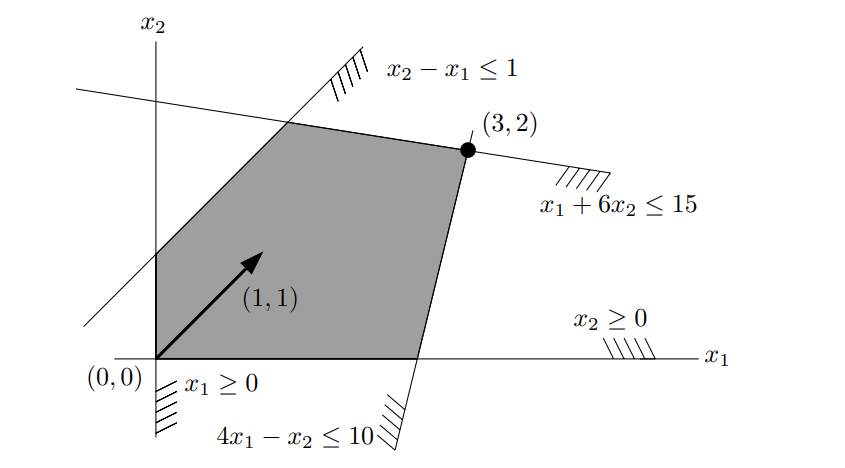
\includegraphics[width=0.8\textwidth]{../img/1.png} % Ajusta el tamaño de la imagen
\label{fig:imagen} % Etiqueta para referenciar la imagen en el texto
\end{figure}
¿Cuál punto de este polígono maximiza el valor de \( x_1 + x_2 \)? El que se encuentra “más alejado en la dirección” del vector \( (1, 1) \) señalado por la flecha; es decir, el punto \( (3, 2) \). La frase “más alejado en la dirección” está entre comillas ya que no es del todo precisa. Para ser más precisos, consideramos una línea perpendicular a la flecha, y pensamos en trasladarla en la dirección de la flecha. Entonces estamos buscando un punto donde la línea en movimiento intersecte nuestro polígono por última vez. (Notemos que la función \( x_1 + x_2 \) es constante en cada línea perpendicular al vector \( (1, 1) \), y a medida que movemos la línea en la dirección de ese vector, el valor de la función aumenta.) Véase la siguiente ilustración:

En un programa lineal general queremos encontrar un vector \( x^* \in \mathbb{R}^n \) que maximice (o minimice) el valor de una función lineal dada entre todos los vectores \( x \in \mathbb{R}^n \) que satisfacen un sistema dado de ecuaciones e inequaciones lineales. La función lineal a maximizar, o a veces minimizar, se llama función objetivo. Tiene la forma \( c^T x = c_1x_1 + \cdots + c_nx_n \), donde \( c \in \mathbb{R}^n \) es un vector dado. \footnote{Aquí consideramos el vector \( c \) como una matriz de tamaño \( n \times 1 \), y así, la expresión \( c^T x \) es un producto de una matriz \( 1 \times n \) y una matriz \( n \times 1 \). Este producto, formalmente hablando, debería ser una matriz \( 1 \times 1 \), pero lo consideramos como un número real.

Algunos lectores podrían preguntarse: Si consideramos a \( c \) como un vector columna, ¿por qué, en el ejemplo anterior, no lo escribimos como una columna o como \( (1, 1)^T \)? Para nosotros, un vector es un \( n \)-tupla de números, y al escribir un vector explícito, separamos los números por comas, como en \( c = (1, 1) \). Solo si un vector aparece en un contexto donde se espera una matriz, es decir, en un producto de matrices, entonces se considera como (o se “convierte a”) una matriz de tamaño \( n \times 1 \). (Sin embargo, a veces declaramos un vector como un vector fila, y entonces se comporta como una matriz \( 1 \times n \).)}

Las ecuaciones e inequaciones lineales en el programa lineal se llaman restricciones. Es común denotar el número de restricciones por \( m \).

Un programa lineal a menudo se escribe usando matrices y vectores, de manera similar a la notación \( Ax = b \) para un sistema de ecuaciones lineales en álgebra lineal. Para simplificar dicha notación, podemos reemplazar cada ecuación en el programa lineal por dos inequaciones opuestas. Por ejemplo, en lugar de la restricción \( x_1 + 3x_2 = 7 \) podemos usar las dos restricciones \( x_1 + 3x_2 \leq 7 \) y \( x_1 + 3x_2 \geq 7 \). Además, la dirección de las inequaciones puede ser invertida cambiando los signos: \( x_1 + 3x_2 \geq 7 \) es equivalente a \( -x_1 - 3x_2 \leq -7 \), y así podemos asumir que todos los signos de las inequaciones son “\(\leq\)”, digamos, con todas las variables apareciendo en el lado izquierdo. Finalmente, minimizar una función objetivo \( c^T x \) es equivalente a maximizar \( -c^T x \), y por lo tanto, siempre podemos convertirlo en un problema de maximización. Después de tales modificaciones, cada programa lineal puede expresarse como sigue:

Maximizar el valor de \( c^T x \)
entre todos los vectores \( x \in \mathbb{R}^n \) que satisfacen \( Ax \leq b \),

donde \( A \) es una matriz real dada \( m \times n \) y \( c \in \mathbb{R}^n \), \( b \in \mathbb{R}^m \) son vectores dados. Aquí la relación \(\leq\) se sostiene para dos vectores de igual longitud si y solo si se sostiene componente a componente.

Cualquier vector \( x \in \mathbb{R}^n \) que satisface todas las restricciones de un programa lineal dado es una solución factible. Cada \( x^* \in \mathbb{R}^n \) que da el valor máximo posible de \( c^T x \) entre todos los \( x \) factibles se llama solución óptima, o simplemente óptimo. En nuestro programa lineal anterior tenemos \( n = 2 \), \( m = 5 \), y \( c = (1, 1) \). La única solución óptima es el vector \( (3, 2) \), mientras que, por ejemplo, \( (2, \frac{3}{2}) \) es una solución factible que no es óptima.

Un programa lineal puede tener en general una única solución óptima, o infinitamente muchas soluciones óptimas, o ninguna en absoluto. Hemos visto una situación con una única solución óptima en el primer ejemplo de un programa lineal. Presentaremos ejemplos de las otras posibles situaciones.
\begin{figure}[H] % La opción [h] indica que la figura debe aparecer aquí
\centering % Centra la imagen en la página
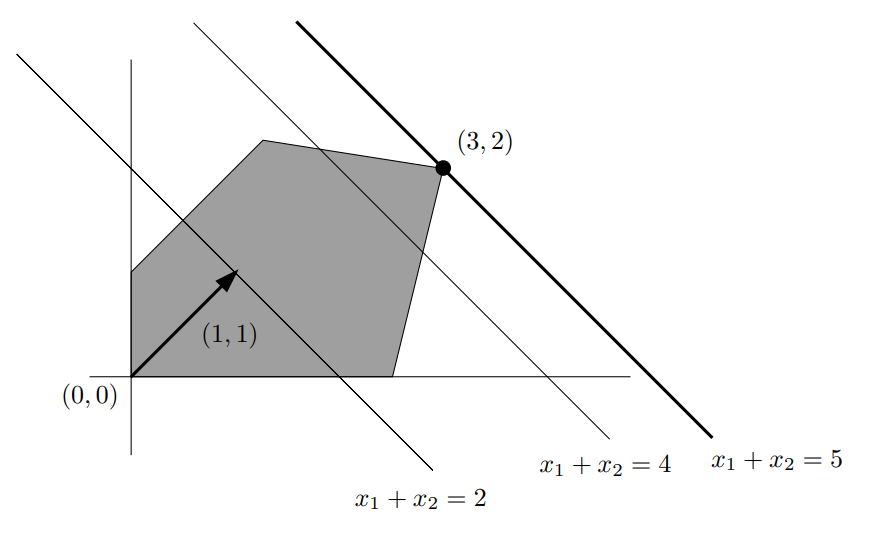
\includegraphics[width=0.8\textwidth]{../img/2.png} % Ajusta el tamaño de la imagen
\label{fig:imagen} % Etiqueta para referenciar la imagen en el texto
\end{figure}

Si invertimos las direcciones de las desigualdades en las restricciones \( x_2 - x_1 \leq 1 \) y \( 4x_1 - x_2 \leq 10 \) en nuestro primer ejemplo, obtenemos un problema de programación lineal que no tiene solución factible, y por lo tanto, tampoco tiene solución óptima:
\begin{figure}[H] % La opción [h] indica que la figura debe aparecer aquí
\centering % Centra la imagen en la página
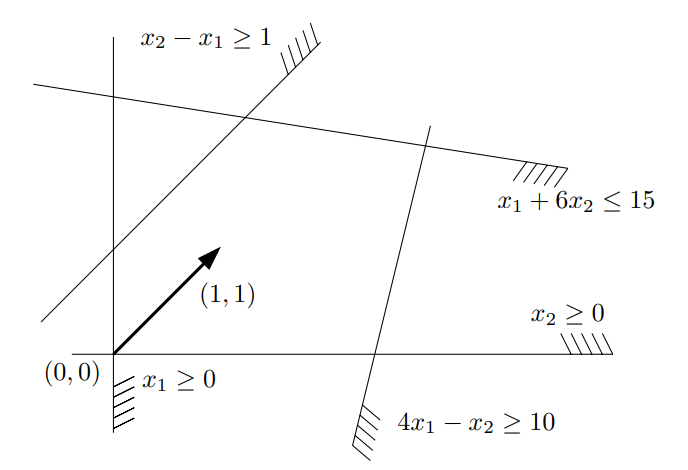
\includegraphics[width=0.8\textwidth]{../img/3.png} % Ajusta el tamaño de la imagen
\label{fig:imagen} % Etiqueta para referenciar la imagen en el texto
\end{figure}

Tal programa lineal se llama no factible. Finalmente, una solución óptima no siempre debe existir, incluso cuando hay soluciones factibles. Esto ocurre cuando la función objetivo puede alcanzar valores arbitrariamente grandes (tal programa lineal se llama sin acotación). Este es el caso cuando eliminamos las restricciones \(4x_1 - x_2 \leq 10\) y \(x_1 + 6x_2 \leq 15\) del ejemplo inicial, como se muestra en la siguiente imagen:

\begin{figure}[H] % La opción [h] indica que la figura debe aparecer aquí
\centering % Centra la imagen en la página
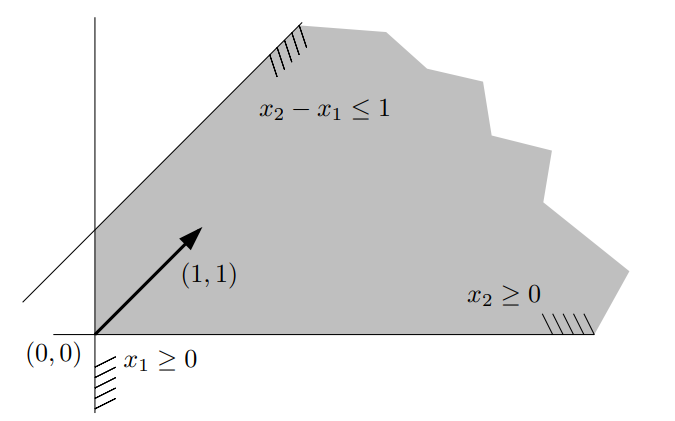
\includegraphics[width=0.8\textwidth]{../img/4.png} % Ajusta el tamaño de la imagen
\label{fig:imagen} % Etiqueta para referenciar la imagen en el texto
\end{figure}

Resumamos: Hemos visto que un programa lineal puede tener una o infinitas soluciones óptimas, pero también puede ser no acotado o no factible. Más adelante demostraremos que no pueden ocurrir otras situaciones.

Hemos resuelto el programa lineal inicial gráficamente. Fue fácil ya que solo hay dos variables. Sin embargo, para un programa lineal con cuatro variables ni siquiera podremos hacer una representación gráfica, y mucho menos encontrar una solución óptima gráficamente. Un programa lineal sustancial en la práctica a menudo tiene varios miles de variables, en lugar de dos o cuatro. Una ilustración gráfica es útil para comprender los conceptos y procedimientos de la programación lineal, pero como método computacional es inútil. A veces, incluso puede ser engañosa, ya que los objetos en dimensiones altas pueden comportarse de manera bastante diferente a lo que sugiere la intuición obtenida en el plano o en el espacio tridimensional.

Uno de los conocimientos clave sobre la programación lineal que se debe recordar para siempre es este:
Un programa lineal es resoluble de manera eficiente, tanto en teoría como en la práctica.
\begin{itemize}
    \item En la práctica, hay varios paquetes de software disponibles. Pueden manejar entradas con varios miles de variables y restricciones. Los programas lineales con una estructura especial, por ejemplo, con un pequeño número de coeficientes distintos de cero en cada restricción, a menudo pueden ser gestionados incluso con un número mucho mayor de variables y restricciones.
    \item En teoría, se han desarrollado algoritmos que resuelven cada programa lineal en un tiempo acotado por una cierta función polinómica del tamaño de la entrada. El tamaño de la entrada se mide como el número total de bits necesarios para escribir todos los coeficientes en la función objetivo y en todas las restricciones.
\end{itemize}
Estas dos afirmaciones resumen los resultados de una larga y ardua investigación, y los métodos eficientes para la programación lineal no son simples.

Para que el conocimiento anterior tenga sentido para siempre, no se debe olvidar qué es un programa lineal, así que lo repetimos una vez más:


\begin{tcolorbox}[colback=white!10!white, colframe=black!75!black, title=Definición de Programa Lineal]
Un programa lineal es el problema de maximizar una función lineal dada sobre el conjunto de todos los vectores que satisfacen un sistema dado de ecuaciones y desigualdades lineales. Cada programa lineal puede transformarse fácilmente a la forma:
\[
\text{maximizar } \mathbf{c}^T \mathbf{x} \text{ sujeto a } \mathbf{A} \mathbf{x} \leq \mathbf{b}.
\]
\end{tcolorbox}

\newpage 
\section{Examples}
\subsection{Diet Problem}
La Oficina de Inspección Nutricional de la UE descubrió recientemente que los platos servidos en el comedor y bar ``Bullneck’s'', como arenques, perritos calientes y hamburguesas estilo casero, no cumplen con las nuevas normativas nutricionales. Su informe mencionó explícitamente la falta de vitaminas A y C y fibra dietética. El propietario y operador de las instalaciones mencionadas está intentando corregir estas deficiencias al agregar platos de acompañamiento vegetales al menú, que pretende preparar a partir de repollo blanco, zanahorias y una reserva de pepinos en vinagre descubiertos en el sótano. La siguiente tabla resume los datos numéricos: la cantidad prescrita de vitaminas y fibra por plato, su contenido en los alimentos y los precios unitarios de los alimentos.
\begin{table}[h]
\centering
\begin{tabularx}{\textwidth}{|l|X|X|X|X|}
\hline
\textbf{Nutriente} & \textbf{Zanahoria} & \textbf{Repollo} & \textbf{Pepino} & \textbf{Requerido por Plato} \\
\hline
\textbf{Vitamina A [mg/kg]} & 35 & 0.5 & 0.5 & 0.5 mg \\
\textbf{Vitamina C [mg/kg]} & 60 & 300 & 10 & 15 mg \\
\textbf{Fibra Dietética [g/kg]} & 30 & 20 & 10 & 4 g \\
\textbf{Precio [€/kg]} & 0.75 & 0.5 & 0.15* & — \\
\hline
\end{tabularx}
\label{tab:datos_nutricionales}
\end{table}

¿Cuál es el precio mínimo adicional por plato para satisfacer los requisitos de la Oficina de Inspección Nutricional? Esta pregunta se puede expresar mediante el siguiente programa lineal:

\begin{equation}
\text{Minimizar} \quad 0.75x_1 + 0.5x_2 + 0.15x_3
\end{equation}

sujeto a
\[
\begin{aligned}
x_1 &\geq 0 \\
x_2 &\geq 0 \\
x_3 &\geq 0 \\
35x_1 + 0.5x_2 + 0.5x_3 &\geq 0.5 \\
60x_1 + 300x_2 + 10x_3 &\geq 15 \\
30x_1 + 20x_2 + 10x_3 &\geq 4
\end{aligned}
\]

La variable \(x_1\) especifica la cantidad de zanahoria (en kg) que se debe agregar a cada plato, y de manera similar para \(x_2\) (repollo) y \(x_3\) (pepino). La función objetivo expresa el precio de la combinación. Las cantidades de zanahoria, repollo y pepino son siempre no negativas, lo que está capturado por las condiciones \(x_1 \geq 0\), \(x_2 \geq 0\), \(x_3 \geq 0\) (si no las incluyéramos, una solución óptima podría tener la cantidad de zanahoria, por ejemplo, negativa, con lo cual aparentemente se ahorraría dinero). Finalmente, las desigualdades en las últimas tres líneas imponen los requisitos de vitaminas A y C y de fibra dietética.

El programa lineal se puede resolver mediante métodos estándar. La solución óptima da un precio de 0.07 € con las siguientes dosis: zanahoria 9.5 g, repollo 38 g y pepino en vinagre 290 g por plato (todo redondeado a dos dígitos significativos). Esto probablemente no pasaría otra ronda de inspección. En realidad, se tendrían que añadir más restricciones, por ejemplo, una sobre la cantidad máxima de pepino en vinagre.
\newpage 

\subsection{Flow in a Network}
Un administrador de una red de computadoras convenció a su empleador de comprar una nueva computadora con un sistema de sonido mejorado. Quiere transferir su colección de música desde una computadora antigua a la nueva, utilizando una red local. La red se ve así:

\begin{figure}[H] % La opción [H] asegura que la figura quede exactamente aquí
\centering % Centra la imagen en la página
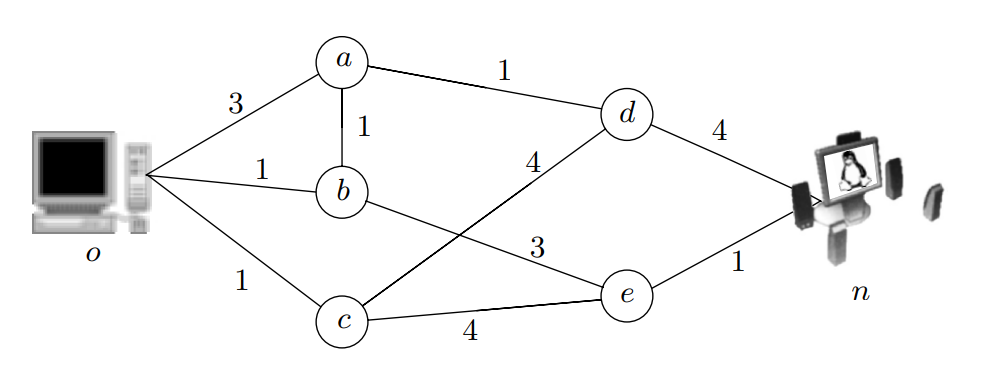
\includegraphics[width=0.8\textwidth]{../img/2.2.png} % Ajusta el tamaño de la imagen
\caption{Descripción de la imagen.} % Descripción de la imagen
\label{fig:imagen} % Etiqueta para referenciar la imagen en el texto
\end{figure}

¿Cuál es la tasa máxima de transferencia desde la computadora \(o\) (antigua) a la computadora \(n\) (nueva)? Los números cercanos a cada enlace de datos especifican la tasa máxima de transferencia de ese enlace (en Mbit/s, por ejemplo). Asumimos que cada enlace puede transferir datos en una dirección, pero no en ambas direcciones simultáneamente. Por lo tanto, por ejemplo, a través del enlace \(ab\) se puede enviar datos desde \(a\) a \(b\) a cualquier tasa desde 0 hasta 1 Mbit/s, o enviar datos desde \(b\) a \(a\) a cualquier tasa de 0 a 1 Mbit/s.

Los nodos \(a\), \(b\), ... , \(e\) no son adecuados para almacenar grandes cantidades de datos, y por lo tanto, todos los datos que ingresan en ellos deben ser enviados de inmediato. A partir de esto, podemos ver que la tasa máxima de transferencia no se puede utilizar en todos los enlaces simultáneamente (considerando el nodo \(a\), por ejemplo). Por lo tanto, debemos encontrar un valor adecuado del flujo de datos para cada enlace de manera que la tasa de transferencia total desde \(o\) hasta \(n\) sea máxima.

Para cada enlace en la red, introducimos una variable. Por ejemplo, \(x_{be}\) especifica la tasa a la que se transfieren datos desde \(b\) hasta \(e\). Aquí \(x_{be}\) también puede ser negativo, lo que significa que el flujo de datos va en la dirección opuesta, de \(e\) a \(b\). (Y así no introducimos otra variable \(x_{eb}\), que correspondería a la tasa de transferencia desde \(e\) a \(b\)). Hay 10 variables: \(x_{oa}\), \(x_{ob}\), \(x_{oc}\), \(x_{ab}\), \(x_{ad}\), \(x_{be}\), \(x_{cd}\), \(x_{ce}\), \(x_{dn}\) y \(x_{en}\).

Establecemos el siguiente programa lineal:

Maximizar \(x_{oa} + x_{ob} + x_{oc}\)

sujeto a las restricciones:
\[
-3 \leq x_{oa} \leq 3, \quad -1 \leq x_{ob} \leq 1, \quad -1 \leq x_{oc} \leq 1,
\]
\[
-1 \leq x_{ab} \leq 1, \quad -1 \leq x_{ad} \leq 1, \quad -3 \leq x_{be} \leq 3,
\]
\[
-4 \leq x_{cd} \leq 4, \quad -4 \leq x_{ce} \leq 4, \quad -4 \leq x_{dn} \leq 4,
\]
\[
-1 \leq x_{en} \leq 1,
\]
\[
x_{oa} = x_{ab} + x_{ad},
\]
\[
x_{ob} + x_{ab} = x_{be},
\]
\[
x_{oc} = x_{cd} + x_{ce},
\]
\[
x_{ad} + x_{cd} = x_{dn},
\]
\[
x_{be} + x_{ce} = x_{en}.
\]

La función objetivo \(x_{oa} + x_{ob} + x_{oc}\) expresa la tasa total a la que se envían datos desde la computadora \(o\). Dado que no se almacenan ni se pierden (esperemos) en ningún lugar, se deben recibir en \(n\) a la misma tasa. Las siguientes 10 restricciones, desde \(-3 \leq x_{oa} \leq 3\) hasta \(-1 \leq x_{en} \leq 1\), limitan las tasas de transferencia a lo largo de los enlaces individuales. Las restricciones restantes indican que todo lo que entra en cada uno de los nodos \(a\) hasta \(e\) debe salir inmediatamente.

La solución óptima de este programa lineal se muestra a continuación: 


\begin{figure}[H] % La opción [h] indica que la figura debe aparecer aquí
\centering % Centra la imagen en la página
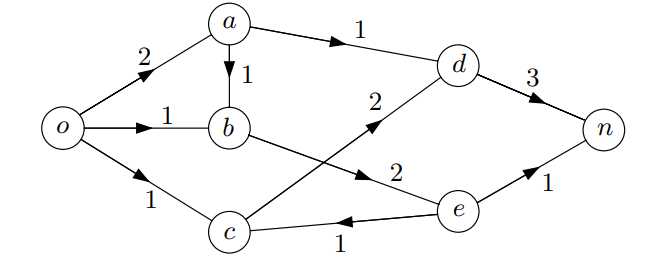
\includegraphics[width=0.8\textwidth]{../img/2.3.png} % Ajusta el tamaño de la imagen
\label{fig:imagen} % Etiqueta para referenciar la imagen en el texto
\end{figure}


El número cercano a cada enlace es la tasa de transferencia en ese enlace, y la flecha determina la dirección del flujo de datos. Nótese que entre \(c\) y \(e\) los datos deben enviarse en la dirección de \(e\) a \(c\), y por lo tanto \(x_{ce} = -1\). El valor óptimo de la función objetivo es 4, y esta es la tasa máxima de transferencia deseada.

En este ejemplo es fácil ver que la tasa de transferencia no puede ser mayor, ya que la capacidad total de todos los enlaces que conectan las computadoras \(o\) y \(a\) con el resto de la red es igual a 4. Este es un caso especial de un notable teorema sobre flujo máximo y corte mínimo, que se discute habitualmente en cursos de algoritmos de grafos (ver también la Sección 8.2).

Nuestro ejemplo de flujo de datos en una red es pequeño y simple. Sin embargo, en la práctica, los flujos se consideran en redes intrincadas, a veces incluso con muchos nodos fuente y nodos sumidero. Estos pueden ser redes eléctricas (flujos de corriente), redes de carreteras o ferrocarriles (flujos de automóviles o trenes), redes telefónicas (flujos de voz o datos), financieras (flujos de dinero), y así sucesivamente. También hay muchas aplicaciones menos obvias de los flujos en redes, por ejemplo, en el procesamiento de imágenes.



\newpage 

\subsection{Ice Cream All Year Round}
La siguiente aplicación de programación lineal también se refiere a la comida (lo cual no debería sorprender, dada la importancia de la comida en la vida y las dificultades para optimizar el sueño o el amor). El fabricante de helados Icicle Works Ltd. necesita establecer un plan de producción para el próximo año. Basado en la historia, encuestas extensivas y observaciones de aves, el departamento de marketing ha elaborado la siguiente predicción de ventas mensuales de helados para el próximo año:

\begin{figure}[H] % La opción [h] indica que la figura debe aparecer aquí
\centering % Centra la imagen en la página
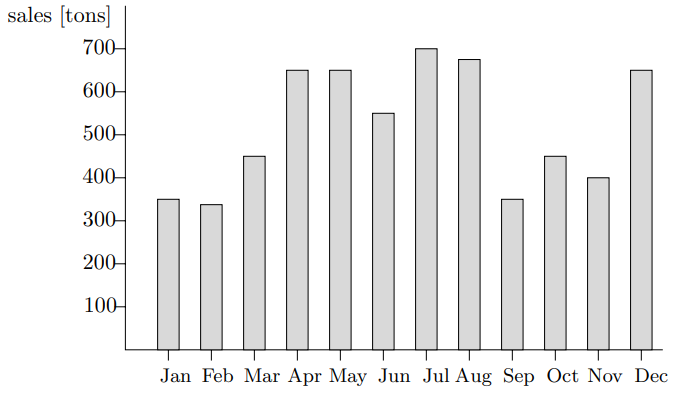
\includegraphics[width=0.8\textwidth]{../img/2.4.png} % Ajusta el tamaño de la imagen
\label{fig:imagen} % Etiqueta para referenciar la imagen en el texto
\end{figure}

Ahora, Icicle Works Ltd. necesita establecer un cronograma de producción para satisfacer estas demandas.
Una solución simple sería producir “justo a tiempo”, lo que significa que todo el helado necesario en el mes \(i\) se produce también en el mes \(i\), \(i = 1, 2, \dots, 12\).
Sin embargo, esto significa que la cantidad producida variaría mucho de un mes a otro, y un cambio en la cantidad producida tiene costos significativos: se deben contratar o despedir trabajadores temporales, ajustar las máquinas, etc.
Por lo tanto, sería mejor distribuir la producción de manera más uniforme a lo largo del año: en los meses de baja demanda, se podrían utilizar las capacidades ociosas de la fábrica para acumular un stock de helado para los meses de alta demanda.
Así, otra solución simple podría ser un cronograma de producción completamente “plano”, con la misma cantidad producida cada mes. Un poco de reflexión revela que dicho cronograma podría no ser factible si queremos terminar el año con un excedente nulo. Pero, incluso si es factible, podría no ser ideal, ya que almacenar helado incurre en un costo no trivial. Parece probable que el mejor cronograma de producción debería estar en algún lugar entre estos dos extremos (producción siguiendo la demanda y producción constante). Queremos un compromiso que minimice el costo total resultante tanto de los cambios en la producción como del almacenamiento de excedentes.

Para formalizar este problema, denotemos la demanda en el mes \(i\) por \(d_i \geq 0\) (en toneladas). Luego, introducimos una variable no negativa \(x_i\) para la producción en el mes \(i\) y otra variable no negativa \(s_i\) para el excedente total almacenado al final del mes \(i\). Para satisfacer la demanda en el mes \(i\), podemos usar la producción del mes \(i\) y el excedente al final del mes \(i-1\):
\[
x_i + s_{i-1} \geq d_i \quad \text{para } i = 1, 2, \dots, 12.
\]
La cantidad \(x_i + s_{i-1} - d_i\) es exactamente el excedente después del mes \(i\), y por lo tanto tenemos
\[
x_i + s_{i-1} - s_i = d_i \quad \text{para } i = 1, 2, \dots, 12.
\]
Suponiendo que inicialmente no hay excedente, establecemos \(s_0 = 0\) (si tomáramos en cuenta la historia de producción, \(s_0\) sería el excedente al final del año anterior). También establecemos \(s_{12} = 0\), a menos que queramos planificar para otro año.

Entre todas las soluciones no negativas a estas ecuaciones, buscamos una que minimice el costo total. Supongamos que cambiar la producción en 1 tonelada de un mes \(i-1\) a un mes \(i\) cuesta €50, y que las instalaciones de almacenamiento para 1 tonelada de helado cuestan €20 por mes. Entonces, el costo total se expresa mediante la función
\[
50 \sum_{i=1}^{12} |x_i - x_{i-1}| + 20 \sum_{i=1}^{12} s_i,
\]
donde establecemos \(x_0 = 0\) (nuevamente, la historia se puede tener en cuenta fácilmente).

Desafortunadamente, esta función de costo no es lineal. Afortunadamente, hay un truco simple pero importante que nos permite hacerla lineal, al precio de introducir variables adicionales.
El cambio en la producción es o un aumento o una disminución. Introduzcamos una variable no negativa \(y_i\) para el aumento del mes \(i-1\) al mes \(i\), y una variable no negativa \(z_i\) para la disminución. Entonces
\[
x_i - x_{i-1} = y_i - z_i \quad \text{y} \quad |x_i - x_{i-1}| = y_i + z_i.
\]
Un cronograma de producción de costo mínimo total se da por una solución óptima del siguiente programa lineal:
\[
\text{Minimizar } \sum_{i=1}^{12} 50y_i + \sum_{i=1}^{12} 50z_i + \sum_{i=1}^{12} 20s_i
\]
sujeto a
\[
x_i + s_{i-1} - s_i = d_i \quad \text{para } i = 1, 2, \dots, 12
\]
\[
x_i - x_{i-1} = y_i - z_i \quad \text{para } i = 1, 2, \dots, 12
\]
\[
x_0 = 0, \quad s_0 = 0, \quad s_{12} = 0
\]
\[
x_i, s_i, y_i, z_i \geq 0 \quad \text{para } i = 1, 2, \dots, 12.
\]
Para ver que una solución óptima (\(s^*, y^*, z^*\)) de este programa lineal define efectivamente un cronograma, necesitamos notar que uno de \(y^*_i\) y \(z^*_i\) tiene que ser cero para todos \(i\), de lo contrario, podríamos reducir ambos y obtener una mejor solución. Esto significa que \(y^*_i + z^*_i\) de hecho es igual al cambio en la producción del mes \(i-1\) al mes \(i\), como se requiere.

En el ejemplo de Icicle Works mencionado anteriormente, este programa lineal produce el siguiente cronograma de producción (mostrado con barras negras; el gráfico de fondo en gris representa las demandas).

\begin{figure}[H] % La opción [h] indica que la figura debe aparecer aquí
\centering % Centra la imagen en la página
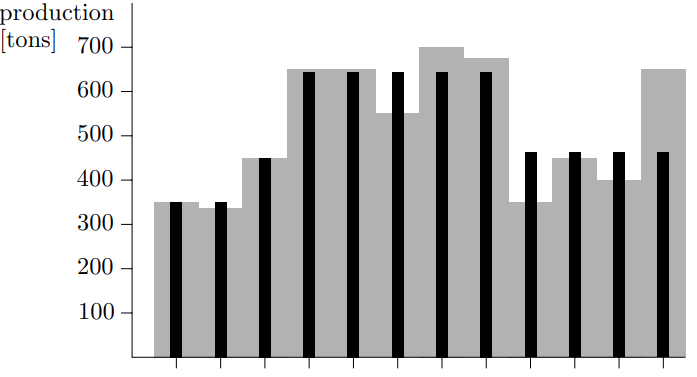
\includegraphics[width=0.8\textwidth]{../img/2.5.png} % Ajusta el tamaño de la imagen
\label{fig:imagen} % Etiqueta para referenciar la imagen en el texto
\end{figure}

A continuación se muestra el cronograma que obtendríamos con costos de almacenamiento cero (es decir, después reemplazando el “20” por “0” en el programa lineal anterior). 
\begin{figure}[H] % La opción [h] indica que la figura debe aparecer aquí
\centering % Centra la imagen en la página
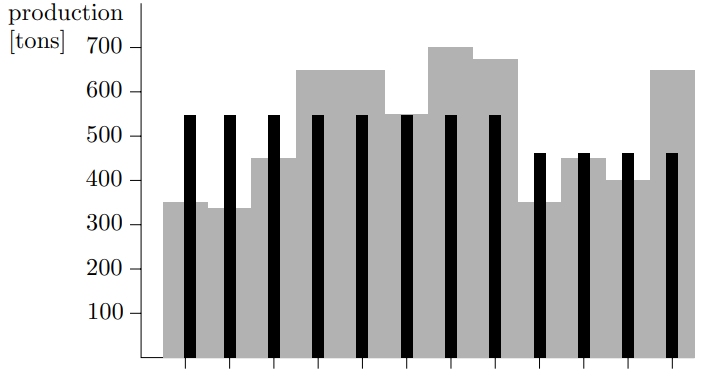
\includegraphics[width=0.8\textwidth]{../img/2.6.png} % Ajusta el tamaño de la imagen
\label{fig:imagen} % Etiqueta para referenciar la imagen en el texto
\end{figure}

El patrón de este ejemplo es bastante general, y muchos problemas de control óptimo pueden resolverse mediante programación lineal de manera similar. Un ejemplo interesante es el juego "Moon Rocket Landing", un juego que fue popular para calculadoras programables (probablemente no lo suficientemente sofisticado como para sobrevivir en la competencia actual). Un módulo lunar con un suministro limitado de combustible está descendiendo verticalmente hacia la superficie lunar bajo la influencia de la gravedad, y en intervalos de tiempo elegidos puede encender sus cohetes para desacelerar el descenso (o incluso para comenzar a volar hacia arriba). El objetivo es aterrizar en la superficie con una velocidad (casi) nula antes de agotar todo el combustible. Se invita al lector a formular un programa lineal adecuado para determinar la cantidad mínima de combustible necesaria para aterrizar, dados los datos de entrada apropiados. Para la formulación de la programación lineal, primero tenemos que discretizar el tiempo (en el juego esto ya se hacía), pero con pasos de tiempo suficientemente cortos esto no hace diferencia en la práctica. Cabe señalar que este problema en particular puede resolverse de manera analítica, con un poco de cálculo (o incluso teoría matemática del control). Pero en situaciones ligeramente más complicadas, una solución analítica está fuera de alcance.

\newpage

\section{La teoría de la Programación Lineal}
\subsection{Ecuación Formal}
En el capítulo introductorio explicamos cómo cada programa lineal puede ser convertido a la forma
\[
\text{maximizar } c^T x \text{ sujeto a } Ax \leq b.
\]
Pero el método simplex requiere una forma diferente, que se suele llamar forma estándar en la literatura. En este libro introducimos un término menos común, pero más descriptivo: forma ecuacional. Se ve así:

\begin{tcolorbox}[colback=white, colframe=black, title=Forma estandar de un Problema de Programación Lineal]
\centering

Maximizar \( c^T x \) \\
sujeto a \( Ax = b \) \\
\( x \geq 0 \).
\end{tcolorbox}

Las restricciones son, por tanto, en parte ecuaciones, y en parte desigualdades de una forma muy especial \( x_j \geq 0 \), \( j = 1, 2, \ldots, n \), llamadas restricciones de no negatividad. (Advertencia: Aunque llamamos a esta forma ecuacional, también contiene desigualdades, y estas no deben ser olvidadas.)

Debemos enfatizar que todas las variables en la forma ecuacional deben satisfacer las restricciones de no negatividad.

En los problemas que encontramos en la práctica, a menudo tenemos restricciones de no negatividad automáticamente, ya que muchas cantidades, como la cantidad de pepino consumido, no pueden ser negativas.


\textbf{Transformación de un programa lineal arbitrario a la forma ecuacional.}
Ilustramos tal transformación para el programa lineal:

\begin{align*}
\text{maximizar } & 3x_1 - 2x_2 \\
\text{sujeto a } & 2x_1 - x_2 \leq 4 \\
& x_1 + 3x_2 \geq 5 \\
& x_2 \geq 0.
\end{align*}

Procedemos de la siguiente manera:

\begin{enumerate}
    \item Para convertir la desigualdad \( 2x_1 - x_2 \leq 4 \) en una ecuación, introducimos una nueva variable \( x_3 \), junto con la restricción de no negatividad \( x_3 \geq 0 \), y reemplazamos la desigualdad considerada por la ecuación
    \[
    2x_1 - x_2 + x_3 = 4.
    \]
    La variable auxiliar \( x_3 \), que no aparecerá en ningún otro lugar del programa lineal transformado, representa la diferencia entre el lado derecho y el lado izquierdo de la desigualdad. Tal variable auxiliar se llama variable de holgura.

    \item Para la siguiente desigualdad \( x_1 + 3x_2 \geq 5 \), primero multiplicamos por \(-1\), lo que invierte la dirección de la desigualdad. Luego introducimos otra variable de holgura \( x_4 \) con la restricción de no negatividad \( x_4 \geq 0 \), y reemplazamos la desigualdad por la ecuación
    \[
    -x_1 - 3x_2 + x_4 = -5.
    \]

    \item No hemos terminado aún: La variable \( x_1 \) en el programa lineal original puede tomar valores positivos y negativos. Introducimos dos nuevas variables no negativas \( y_1 \) y \( z_1 \), \( y_1 \geq 0 \), \( z_1 \geq 0 \), y sustituimos por \( x_1 \) la diferencia \( y_1 - z_1 \) en todas partes. La variable \( x_1 \) en sí desaparece. La forma ecuacional resultante de nuestro programa lineal es
    \[
    \text{maximizar } 3y_1 - 3z_1 - 2x_2
    \]
    sujeto a
    \[
    2y_1 - 2z_1 - x_2 + x_3 = 4
    \]
    \[
    -y_1 + z_1 - 3x_2 + x_4 = -5
    \]
    \[
    y_1 \geq 0, \; z_1 \geq 0, \; x_2 \geq 0, \; x_3 \geq 0, \; x_4 \geq 0.
    \]
\end{enumerate}

    Para cumplir completamente con las convenciones de la forma ecuacional, deberíamos renombrar ahora las variables a \( x_1, x_2, \ldots, x_5 \).

    El procedimiento presentado convierte un programa lineal arbitrario con \( n \) variables y \( m \) restricciones en un programa lineal en forma ecuacional con a lo sumo \( m + 2n \) variables y \( m \) ecuaciones (y, por supuesto, restricciones de no negatividad para todas las variables).

    \textbf{Geometría de un programa lineal en forma ecuacional.} Consideremos un programa lineal en forma ecuacional:
    \[
    \text{Maximizar } c^T x \text{ sujeto a } Ax = b, \; x \geq 0.
    \]
    Como se deriva en álgebra lineal, el conjunto de todas las soluciones del sistema \( Ax = b \) es un subespacio afín \( F \) del espacio \( \mathbb{R}^n \). Por lo tanto, el conjunto de todas las soluciones factibles del programa lineal es la intersección de \( F \) con el ortante no negativo, que es el conjunto de todos los puntos en \( \mathbb{R}^n \) con todas las coordenadas no negativas.\footnote{En el plano (\(n = 2\)) este conjunto se llama el cuadrante no negativo; en \(\mathbb{R}^3\) es el octante no negativo, y el nombre ortante se utiliza para una dimensión arbitraria.
}
El siguiente gráfico ilustra la geometría de las soluciones factibles para un programa lineal con \( n = 3 \) variables y \( m = 1 \) ecuación, a saber, la ecuación \( x_1 + x_2 + x_3 = 1 \):
\newpage 

\begin{figure}[H] % La opción [h] indica que la figura debe aparecer aquí
\centering % Centra la imagen en la página
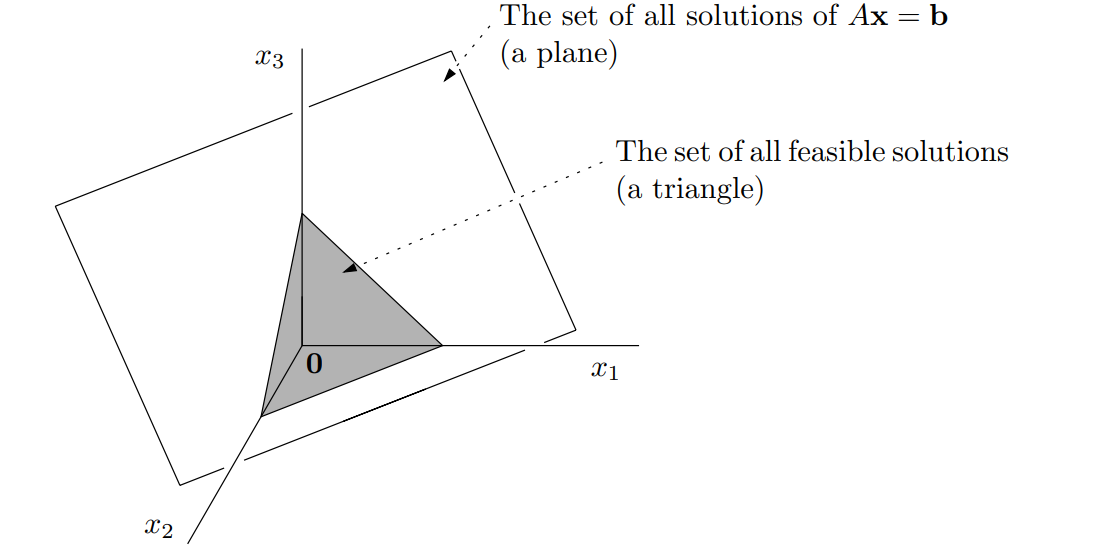
\includegraphics[width=0.8\textwidth]{../img/5.png} % Ajusta el tamaño de la imagen
\label{fig:imagen} % Etiqueta para referenciar la imagen en el texto
\end{figure}


(En casos interesantes, usualmente tenemos más de 3 variables y no se puede dibujar una imagen.)

Una limpieza preliminar. Ahora hablaremos sobre soluciones del sistema \( Ax = b \). Con esto nos referimos a soluciones reales arbitrarias, cuyos componentes pueden ser positivos, negativos o cero. Esto no es lo mismo que soluciones factibles del programa lineal considerado, ya que una solución factible debe satisfacer \( Ax = b \) y tener todos los componentes no negativos.

Si cambiamos el sistema \( Ax = b \) mediante alguna transformación que preserve el conjunto de soluciones, como una operación de fila en la eliminación de Gauss, esto no influye ni en las soluciones factibles ni en las soluciones óptimas del programa lineal. Esto se utilizará ampliamente en el método simplex.

Supuesto: Consideraremos solo programas lineales en forma ecuacional tales que
\begin{itemize}
    \item el sistema de ecuaciones \( Ax = b \) tenga al menos una solución, y
    \item las filas de la matriz \( A \) sean linealmente independientes.
\end{itemize}

Como explicación de este supuesto, necesitamos recordar algunos hechos de álgebra lineal. Verificar si el sistema \( Ax = b \) tiene una solución es fácil mediante eliminación de Gauss, y si no hay solución, el programa lineal considerado tampoco tiene solución factible, por lo que podemos descartarlo.

Si el sistema \( Ax = b \) tiene una solución y si alguna fila de \( A \) es una combinación lineal de las otras filas, entonces la ecuación correspondiente es redundante y puede eliminarse del sistema sin cambiar el conjunto de soluciones. Por lo tanto, podemos suponer que la matriz \( A \) tiene \( m \) filas linealmente independientes y (por lo tanto) rango \( m \).


\newpage 
\subsection{Soluciones factibles básicas}
Entre todas las soluciones factibles de un programa lineal, se concede un estatus privilegiado a las llamadas soluciones básicas factibles. En esta sección consideraremos estas soluciones solo para programas lineales en forma ecuacional. Observemos nuevamente la imagen del conjunto de soluciones factibles para un programa lineal con \( n = 3 \), \( m = 1 \):

\begin{figure}[H] % La opción [h] indica que la figura debe aparecer aquí
\centering % Centra la imagen en la página
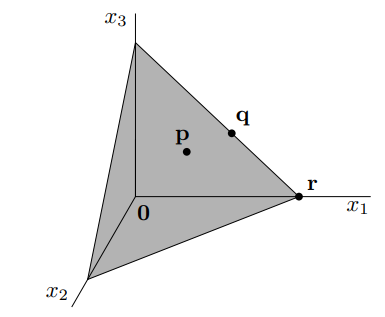
\includegraphics[width=0.5\textwidth]{../img/6.png} % Ajusta el tamaño de la imagen
\label{fig:imagen} % Etiqueta para referenciar la imagen en el texto
\end{figure}

Entre las soluciones factibles \( p \), \( q \) y \( r \), solo \( r \) es básica. Expresado geométricamente y de manera muy informal, una solución básica factible es un vértice (esquina, pico) del conjunto de soluciones factibles. Formularemos esta descripción geométrica de una solución básica factible más adelante (ver Teorema 4.4.1).

La definición que presentamos a continuación resulta ser equivalente, pero se ve bastante diferente. Requiere que, a grosso modo, una solución básica factible tenga un número suficiente de componentes cero. Antes de enunciarla, introducimos un nuevo conjunto de notación.

En esta sección, \( A \) es siempre una matriz con \( m \) filas y \( n \) columnas (\( n \geq m \)), de rango \( m \). Para un subconjunto \( B \subseteq \{1, 2, \ldots, n\} \), denotamos \( A_B \) como la matriz formada por las columnas de \( A \) cuyos índices pertenecen a \( B \). Por ejemplo, para
\[
A =
\begin{bmatrix}
1 & 5 & 3 & 4 & 6 \\
0 & 1 & 3 & 5 & 6
\end{bmatrix}
\]
y \( B = \{2, 4\} \), tenemos
\[
A_B =
\begin{bmatrix}
5 & 4 \\
1 & 5
\end{bmatrix}.
\]

Usaremos una notación similar para los vectores; por ejemplo, para \( x = (3, 5, 7, 9, 11) \) y \( B = \{2, 4\} \), tenemos \( x_B = (5, 9) \).

Ahora estamos listos para enunciar una definición formal.

\begin{tcolorbox}[colback=white, colframe=black, title=Definición de Solución Básica Factible]
Una solución básica factible del programa lineal
\[
\text{maximizar } c^T x \text{ sujeto a } Ax = b \text{ y } x \geq 0
\]
es una solución factible \( x \in \mathbb{R}^n \) para la cual existe un conjunto \( B \) de \( m \) elementos con \( B \subseteq \{1, 2, \ldots, n\} \) tal que
\begin{itemize}
    \item la matriz (cuadrada) \( A_B \) es no singular, es decir, las columnas indexadas por \( B \) son linealmente independientes, y
    \item \( x_j = 0 \) para todo \( j \notin B \).
\end{itemize}
\end{tcolorbox}

Por ejemplo, \( x = (0, 2, 0, 1, 0) \) es una solución básica factible para

\[
A = \begin{pmatrix}
1 & 5 & 3 & 4 & 6 \\
0 & 1 & 3 & 5 & 6
\end{pmatrix},
\quad b = \begin{pmatrix}
14 \\
7
\end{pmatrix}
\]

con \( B = \{2, 4\} \).

Si se fija tal conjunto \( B \), llamamos a las variables \( x_j \) con \( j \in B \) las variables básicas, mientras que las variables restantes se llaman no básicas. Así, podemos decir brevemente que todas las variables no básicas son cero en una solución básica factible.

Cabe notar que la definición no considera en absoluto el vector \( c \), y por lo tanto las soluciones básicas factibles dependen únicamente de \( A \) y \( b \).

Para algunas consideraciones, es conveniente reformular la definición de una solución básica factible un poco.

\textbf{Lema 4.2.1.} Una solución factible \( x \) de un programa lineal en forma ecuacional es básica si y solo si las columnas de la matriz \( A_K \) son linealmente independientes, donde \( K = \{j \in \{1, 2, \ldots, n\} : x_j > 0\} \).

\textbf{Prueba.} Una de las implicaciones es obvia: Si \( x \) es una solución básica factible y \( B \) es el conjunto correspondiente de \( m \) elementos como en la definición, entonces \( K \subseteq B \) y por lo tanto las columnas de la matriz \( A_K \) son linealmente independientes.

A la inversa, sea \( x \) factible y tales que las columnas de \( A_K \) son linealmente independientes. Si \( |K| = m \), entonces podemos tomar simplemente \( B = K \). De lo contrario, para \( |K| < m \), extendemos \( K \) a un conjunto de \( m \) elementos \( B \) añadiendo \( m - |K| \) índices más de modo que las columnas de \( A_B \) sean linealmente independientes. Este es un hecho estándar de álgebra lineal, que puede ser verificado usando el algoritmo descrito a continuación. Inicialmente fijamos el conjunto actual \( B \) en \( K \), y repetimos el siguiente paso: Si \( A \) tiene una columna que no está en el espacio lineal de las columnas de \( A_B \), añadimos el índice de tal columna a \( B \). Tan pronto como este paso ya no sea posible, es decir, todas las columnas de \( A \) están en el espacio lineal de las columnas de \( B \), se ve fácilmente que las columnas de \( A_B \) constituyen una base del espacio de columnas de \( A \). Dado que \( A \) tiene rango \( m \), tenemos \( |B| = m \) como se necesita.

\textbf{Proposición 4.2.2.} Una solución básica factible está determinada de manera única por el conjunto \( B \). Es decir, para cada conjunto de \( m \) elementos \( B \subseteq \{1, 2, \ldots, n\} \) con \( A_B \) no singular, existe como máximo una solución factible \( x \in \mathbb{R}^n \) con \( x_j = 0 \) para todo \( j \notin B \).

Debemos destacar de inmediato que una única solución básica factible puede obtenerse a partir de muchos conjuntos diferentes \( B \).

\textbf{Prueba de la Proposición 4.2.2.} Para que \( x \) sea factible debemos tener \( A x = b \). El lado izquierdo puede reescribirse como \( A x = A_B x_B + A_N x_N \), donde \( N = \{1, 2, \ldots, n\} \setminus B \). Para que \( x \) sea una solución básica factible, el vector \( x_N \) de variables no básicas debe ser igual a 0, y así el vector \( x_B \) de variables básicas satisface \( A_B x_B = b \). Y aquí usamos el hecho de que \( A_B \) es una matriz cuadrada no singular: El sistema \( A_B x_B = b \) tiene exactamente una solución \( \tilde{x}_B \). Si todos los componentes Si los componentes de \( \tilde{x}_B \) son no negativos, entonces tenemos exactamente una solución básica factible para el conjunto \( B \) considerado (modificamos \( \tilde{x}_B \) añadiendo ceros), y en caso contrario, no tenemos ninguna.

Introducimos la siguiente terminología: Llamamos a un conjunto de \( m \) elementos \( B \subseteq \{1, 2, \ldots, n\} \) con \( A_B \) no singular una base. Si, además, \( B \) determina una solución básica factible, o en otras palabras, si la solución única del sistema \( A_B x_B = b \) es no negativa, entonces llamamos a \( B \) una base factible.

El siguiente teorema trata sobre la existencia de soluciones óptimas y, además, muestra que basta con buscar estas soluciones únicamente entre las soluciones básicas factibles.

\textbf{Teorema 4.2.3.} Consideremos un programa lineal en forma ecuacional:

\[
\text{maximizar } c^T x \text{ sujeto a } A x = b, \; x \geq 0.
\]

(i) (“Las soluciones óptimas pueden no existir solo por razones obvias.”) Si hay al menos una solución factible y la función objetivo está acotada superiormente en el conjunto de todas las soluciones factibles, entonces existe una solución óptima.

(ii) Si existe una solución óptima, entonces hay una solución básica factible que es óptima.

No es necesario proporcionar una prueba para la lectura adicional y la dejaremos al final de esta sección. El teorema también se sigue de la corrección del método simplex, que se discutirá en el próximo capítulo.

El teorema recién enunciado implica un algoritmo finito, aunque totalmente poco práctico, para resolver programas lineales en forma ecuacional. Consideramos todos los subconjuntos de \( m \) elementos \( B \subseteq \{1, 2, \ldots, n\} \) uno por uno, y para cada uno de ellos verificamos si es una base factible, resolviendo un sistema de ecuaciones lineales (obtenemos a lo sumo una solución básica factible para cada \( B \) mediante la Proposición 4.2.2). Luego calculamos el máximo de la función objetivo sobre todas las soluciones básicas factibles encontradas de esta manera.

Hablando estrictamente, este algoritmo no funciona si la función objetivo es no acotada. Formular una variante del algoritmo que funcione correctamente incluso en este caso, es decir, que reporte que el programa lineal es no acotado, lo dejamos como ejercicio. Pronto discutiremos el método simplex, considerablemente más eficiente, y allí mostraremos en detalle cómo tratar con la no acotación.

Debemos considerar \( \binom{n}{m} \) conjuntos \( B \) en el algoritmo anterior. Por ejemplo, para \( n = 2m \), la función \( \binom{2m}{m} \) crece aproximadamente como \( 4^m \), es decir, exponencialmente, y esto es demasiado incluso para \( m \) moderadamente grande.

Como veremos en el Capítulo 5, el método simplex también pasa por soluciones básicas factibles, pero de una manera más inteligente. Camina de una a otra mientras mejora el valor de la función objetivo todo el tiempo, hasta que alcanza una solución óptima.

Resumamos los principales hallazgos de esta sección.

\begin{tcolorbox}[colback=white, colframe=black, title=Conclusión de la Sección]
Un programa lineal en forma ecuacional o estandar tiene un número finito de soluciones básicas factibles, y si es factible y acotado, entonces al menos una de las soluciones básicas factibles es óptima.

En consecuencia, cualquier programa lineal que sea factible y acotado tiene una solución óptima.
\end{tcolorbox}
\newpage 
\subsection{ABC de la convexidad y los poliedros convexos.}
La convexidad es una de las nociones fundamentales en toda la matemática, y en la teoría de la programación lineal se encuentra de manera muy natural. Aquí recordamos la definición y presentamos algunas de las nociones y resultados más básicos, que, al menos, ayudan a obtener una mejor intuición sobre la programación lineal. Por otro lado, la programación lineal puede presentarse sin estos conceptos, y en cursos concisos generalmente no hay tiempo para tales materiales. En consecuencia, esta sección y la siguiente están destinadas a ser material adicional, y el resto del libro debería ser mayormente accesible sin ellos.

\begin{tcolorbox}[colback=white!10!white, colframe=black, title=Definición de Conjunto Convexo]
Un conjunto \( X \subseteq \mathbb{R}^n \) es convexo si para cada par de puntos \( x, y \in X \) también contiene el segmento \( xy \). Expresado de otra manera, para cada \( x, y \in X \) y cada \( t \in [0, 1] \) tenemos \( tx + (1-t)y \in X \).
\end{tcolorbox}

Una breve explicación puede ser útil: \( tx + (1-t)y \) es el punto en el segmento \( xy \) a una distancia \( t \) de \( y \) y a una distancia \( 1-t \) de \( x \), si tomamos la longitud del segmento como distancia unitaria.

Aquí hay algunos ejemplos de conjuntos convexos y no convexos en el plano: 

\begin{figure}[H] % La opción [h] indica que la figura debe aparecer aquí
\centering % Centra la imagen en la página
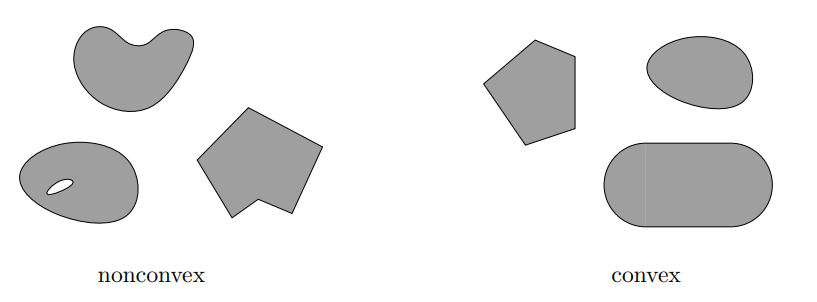
\includegraphics[width=0.8\textwidth]{../img/7.png} % Ajusta el tamaño de la imagen
\label{fig:imagen} % Etiqueta para referenciar la imagen en el texto
\end{figure}

El conjunto convexo en la parte inferior derecha de esta imagen, un estadio, es digno de recordar, ya que a menudo es un contraejemplo a afirmaciones sobre conjuntos convexos que pueden parecer obvias a primera vista pero son falsas.

En cálculo se trabaja principalmente con funciones convexas. Ambas nociones, conjuntos convexos y funciones convexas, están estrechamente relacionadas: Por ejemplo, una función real \( f: \mathbb{R} \to \mathbb{R} \) es convexa si y solo si su epígrafe, es decir, el conjunto \( \{(x, y) \in \mathbb{R}^2 : y \geq f(x)\} \), es un conjunto convexo en el plano. En general, una función \( f: X \to \mathbb{R} \) se llama convexa si para cada \( x, y \in X \) y cada \( t \in [0, 1] \) se cumple:
\[
f(tx + (1-t)y) \leq t f(x) + (1-t) f(y).
\]
La función se llama estrictamente convexa si la desigualdad es estricta para todo \( x \neq y \).

\textbf{Recubrimiento convexo y combinaciones convexas.} Se observa fácilmente que la intersección de una colección arbitraria de conjuntos convexos es nuevamente un conjunto convexo. Esto nos permite definir el recubrimiento convexo.

Sea \( X \subset \mathbb{R}^n \) un conjunto. El recubrimiento convexo de \( X \) es la intersección de todos los conjuntos convexos que contienen a \( X \). Por lo tanto, es el conjunto convexo más pequeño que contiene a \( X \), en el sentido de que cualquier conjunto convexo que contenga a \( X \) también contiene su recubrimiento convexo.

\begin{figure}[H] % La opción [h] indica que la figura debe aparecer aquí
\centering % Centra la imagen en la página
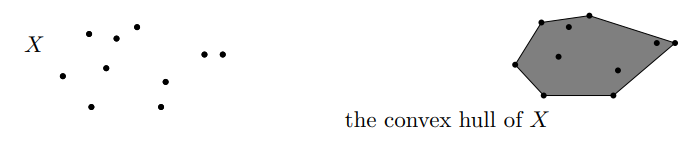
\includegraphics[width=0.8\textwidth]{../img/8.png} % Ajusta el tamaño de la imagen
\label{fig:imagen} % Etiqueta para referenciar la imagen en el texto
\end{figure}

Esta no es una definición muy constructiva. El recubrimiento convexo también se puede describir usando combinaciones convexas, de manera similar a la descripción del espacio lineal de un conjunto de vectores utilizando combinaciones lineales. Sea \( x_1, x_2, \ldots, x_m \) puntos en \( \mathbb{R}^n \). Cada punto de la forma
\[
t_1x_1 + t_2x_2 + \cdots + t_mx_m, \text{ donde } t_1, t_2, \ldots, t_m \geq 0 \text{ y } \sum_{i=1}^m t_i = 1,
\]
se llama una combinación convexa de \( x_1, x_2, \ldots, x_m \). Una combinación convexa es, por lo tanto, un tipo particular de combinación lineal, en la cual los coeficientes son no negativos y suman 1.

\textbf{Combinaciones Convexas}

Las combinaciones convexas de dos puntos \( x \) y \( y \) tienen la forma \( tx + (1 - t)y \), con \( t \in [0, 1] \). Como se mencionó después de la definición de un conjunto convexo, estas combinaciones llenan exactamente el segmento \( xy \). Es fácil, pero instructivo, mostrar que todas las combinaciones convexas de tres puntos \( x \), \( y \), \( z \) llenan exactamente el triángulo \( xyz \) (a menos que los puntos sean colineales).

\textbf{Lema 4.3.1.} El casco convexo \( C \) de un conjunto \( X \subseteq \mathbb{R}^n \) es igual al conjunto
\[
\tilde{C} = \left\{ \sum_{i=1}^{m} t_i x_i \mid m \geq 1, \, x_1, \ldots, x_m \in X, \, t_1, \ldots, t_m \geq 0, \, \sum_{i=1}^{m} t_i = 1 \right\}
\]
de todas las combinaciones convexas de un número finito de puntos de \( X \).

\textbf{Prueba.} Primero demostramos por inducción en \( m \) que cada combinación convexa debe estar en el casco convexo \( C \). Para \( m = 1 \) es obvio y para \( m = 2 \) sigue directamente de la convexidad de \( C \).

Sea \( m \geq 3 \) y sea \( x = t_1 x_1 + \cdots + t_m x_m \) una combinación convexa de puntos de \( X \). Si \( t_m = 1 \), entonces tenemos \( x = x_m \in C \). Para \( t_m < 1 \), pongamos \( t_i = \frac{t_i}{1 - t_m} \), para \( i = 1, 2, \ldots, m - 1 \). Entonces \( x = t_1 x_1 + \cdots + t_{m-1} x_{m-1} \) es una combinación convexa de los puntos \( x_1, \ldots, x_{m-1} \) (los \( t_i \) suman 1), y por la hipótesis de inducción \( x \in C \). Así que \( x = (1 - t_m)x + t_m x_m \) es una combinación convexa de dos puntos del conjunto (convexo) \( C \) y, como tal, también está en \( C \). Por lo tanto, hemos demostrado que \( \tilde{C} \subseteq C \). Para la inclusión inversa, basta con probar que \( \tilde{C} \) es convexo, es decir, verificar que siempre que \( x, y \in \tilde{C} \) sean dos combinaciones convexas y \( t \in (0, 1) \), entonces \( tx + (1 - t)y \) es nuevamente una combinación convexa. Esto es directo y nos tomamos la libertad de omitir más detalles.

\textbf{Hiperplanos, Semiespacios y Poliedros}

Recordemos que un hiperplano en \( \mathbb{R}^n \) es un subespacio afín de dimensión \( n - 1 \). En otras palabras, es el conjunto de todas las soluciones de una sola ecuación lineal de la forma
\[
a_1 x_1 + a_2 x_2 + \cdots + a_n x_n = b,
\]
donde \( a_1, a_2, \ldots, a_n \) no son todos cero. Los hiperplanos en \( \mathbb{R}^2 \) son líneas y los hiperplanos en \( \mathbb{R}^3 \) son planos ordinarios.

Un hiperplano divide \( \mathbb{R}^n \) en dos semiespacios y constituye su frontera común. Para el hiperplano con ecuación \( a_1 x_1 + a_2 x_2 + \cdots + a_n x_n = b \), los dos semiespacios tienen la siguiente expresión analítica:
\[
\left\{ x \in \mathbb{R}^n \mid a_1 x_1 + a_2 x_2 + \cdots + a_n x_n \leq b \right\}
\]
y
\[
\left\{ x \in \mathbb{R}^n \mid a_1 x_1 + a_2 x_2 + \cdots + a_n x_n \geq b \right\}.
\]
Más exactamente, estos son semiespacios cerrados que contienen su frontera.
\begin{center}
\begin{tcolorbox}[sharp corners=south, colback=white, colframe=black, boxrule=0.8mm, width=0.9\textwidth]

    
Un poliedro convexo es una intersección de un número finito de semiespacios cerrados en \( \mathbb{R}^n \).
\end{tcolorbox}
\end{center}
Un semiespacio es claramente convexo, y por lo tanto, la intersección de semiespacios también es convexa. Así, los poliedros convexos tienen el atributo de ser convexos por derecho.

Un disco en el plano es un conjunto convexo, pero no es un poliedro convexo (porque, a grandes rasgos, un poliedro convexo debe ser "con aristas"... pero intenta probar esto formalmente).

Un semiespacio es el conjunto de todas las soluciones de una sola desigualdad lineal (con al menos un coeficiente no nulo de alguna variable \(x_j\)). El conjunto de todas las soluciones de un sistema de un número finito de desigualdades lineales, también conocido como el conjunto de todas las soluciones factibles de un programa lineal, es geométricamente la intersección de un número finito de semiespacios, es decir, un poliedro convexo. (Quizás también deberíamos mencionar que un hiperplano es la intersección de dos semiespacios, por lo que las restricciones pueden ser tanto desigualdades como ecuaciones.)

Debemos señalar que un poliedro convexo puede ser no acotado, ya que, por ejemplo, un único semiespacio también es un poliedro convexo. Un poliedro convexo acotado, es decir, uno que puede ser contenido dentro de una esfera lo suficientemente grande, se llama un poliedro convexo.

La dimensión de un poliedro convexo \(P \subseteq \mathbb{R}^n\) es la dimensión mínima de un subespacio afín que contiene \(P\). Equivalente a esto, es el valor máximo \(d\) para el cual \(P\) contiene puntos \(x_0, x_1, \ldots, x_d\) tales que el \(d\)-tuplo de vectores \((x_1 - x_0, x_2 - x_0, \ldots, x_d - x_0)\) es linealmente independiente.

El conjunto vacío también es un poliedro convexo, y su dimensión generalmente se define como \(-1\).

Todos los polígonos convexos en el plano son poliedros convexos bidimensionales. Varios tipos de poliedros convexos tridimensionales se enseñan en las escuelas secundarias y decoran los gabinetes matemáticos, como cubos, cajas, pirámides, o incluso dodecaedros regulares, que también se pueden encontrar como calendarios de escritorio.

Ejemplos simples de poliedros convexos de dimensión arbitraria \(n\) son:
\begin{itemize}
    \item El cubo \(n\)-dimensional \([-1, 1]^n\), que se puede escribir como la intersección de \(2^n\) semiespacios (¿cuáles?):
\end{itemize}
\begin{figure}[H] % La opción [h] indica que la figura debe aparecer aquí
\centering % Centra la imagen en la página
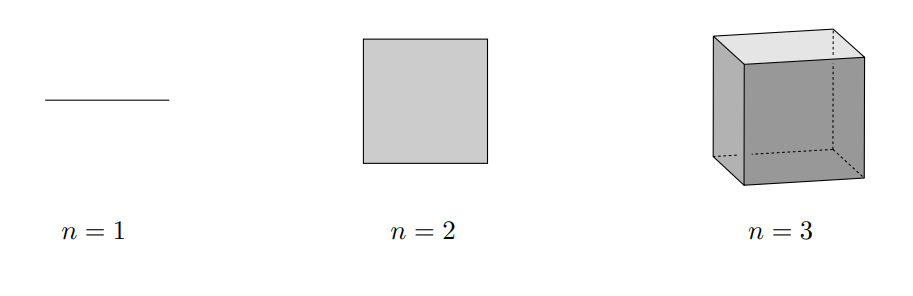
\includegraphics[width=0.8\textwidth]{../img/9.png} % Ajusta el tamaño de la imagen
\label{fig:imagen} % Etiqueta para referenciar la imagen en el texto
\end{figure}
\begin{itemize}
\item El poliedro cruzado \(n\)-dimensional \(\{ x \in \mathbb{R}^n : |x_1| + |x_2| + \cdots + |x_n| \leq 1 \}\):
Para \(n = 3\) obtenemos el octaedro regular. Para expresar el poliedro cruzado \(n\)-dimensional como una intersección de semiespacios necesitamos \(2^n\) semiespacios (¿puedes encontrarlos?).
\end{itemize}

\begin{figure}[H] % La opción [h] indica que la figura debe aparecer aquí
\centering % Centra la imagen en la página
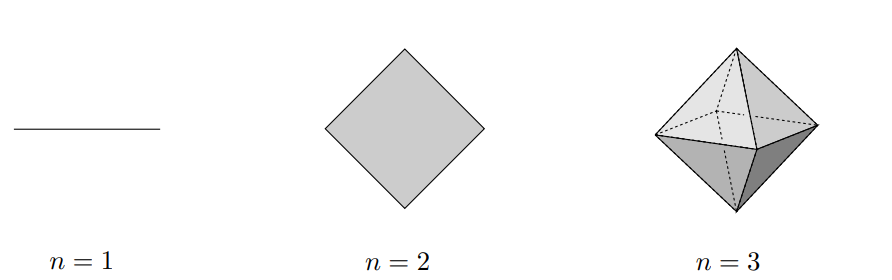
\includegraphics[width=0.8\textwidth]{../img/10.png} % Ajusta el tamaño de la imagen
\label{fig:imagen} % Etiqueta para referenciar la imagen en el texto
\end{figure}

\begin{itemize}
\item El simplex regular \(n\)-dimensional.

\begin{figure}[H] % La opción [h] indica que la figura debe aparecer aquí
\centering % Centra la imagen en la página
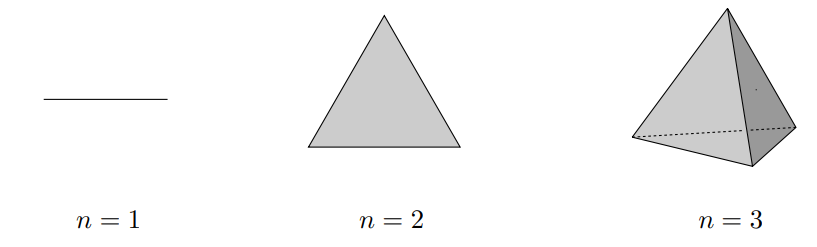
\includegraphics[width=0.8\textwidth]{../img/11.png} % Ajusta el tamaño de la imagen
\label{fig:imagen} % Etiqueta para referenciar la imagen en el texto
\end{figure}

se puede definir de una manera bastante simple y elegante como un subconjunto de \(\mathbb{R}^{n+1}\):
\[
\{ x \in \mathbb{R}^{n+1} : x_1, x_2, \ldots, x_{n+1} \geq 0, \; x_1 + x_2 + \cdots + x_{n+1} = 1 \}.
\]
Observamos que este es exactamente el conjunto de todas las soluciones factibles del programa lineal con la única ecuación \(x_1 + x_2 + \cdots + x_{n+1} = 1\) y las restricciones de no negatividad; ver la imagen en la Sección 4.1. En general, cualquier poliedro convexo \(n\)-dimensional limitado por \(n+1\) hiperplanos se llama simplex.
\end{itemize}

Muchos ejemplos interesantes de poliedros convexos se obtienen como conjuntos de soluciones factibles de programas lineales naturales. Por ejemplo, la relajación LP del problema de emparejamiento de peso máximo (Sección 3.2) para un grafo bipartito completo lleva al poliedro de Birkhoff. Las propiedades geométricas de tales poliedros a menudo están relacionados con propiedades de objetos combinatorios y con soluciones de
problemas de optimización combinatoria de una manera interesante.

\newpage 
\subsection{Vertices y Soluciones Basicas factibles}

Un vértice de un poliedro convexo puede ser pensado como una "punta" o "espina". Por ejemplo, un cubo tridimensional tiene 8 vértices, y un octaedro regular tiene 6 vértices.

Matemáticamente, un vértice se define como un punto donde alguna función lineal alcanza un máximo único. Así, un punto \( v \) se llama vértice de un poliedro convexo \( P \subseteq \mathbb{R}^n \) si \( v \in P \) y existe un vector no nulo \( c \in \mathbb{R}^n \) tal que \( c^T v > c^T y \) para todo \( y \in P \setminus \{v\} \). Geométricamente, esto significa que el hiperplano \( \{ x \in \mathbb{R}^n : c^T x = c^T v \} \) toca el poliedro \( P \) exactamente en \( v \).


\begin{figure}[H] % La opción [h] indica que la figura debe aparecer aquí
\centering % Centra la imagen en la página
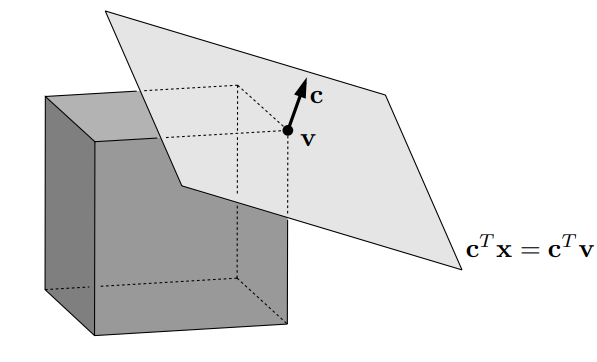
\includegraphics[width=0.8\textwidth]{../img/12.png} % Ajusta el tamaño de la imagen
\label{fig:imagen} % Etiqueta para referenciar la imagen en el texto
\end{figure}
Los poliedros tridimensionales no solo tienen vértices, sino también aristas y caras. Un poliedro general \( P \subseteq \mathbb{R}^n \) de dimensión \( n \) puede tener vértices, aristas, caras de 2 dimensiones, caras de 3 dimensiones, hasta caras de \( (n-1) \) dimensiones. Se definen de la siguiente manera: un subconjunto \( F \subseteq P \) es una cara de \( k \) dimensiones de un poliedro convexo \( P \) si \( F \) tiene dimensión \( k \) y existe un vector no nulo \( c \in \mathbb{R}^n \) y un número \( z \in \mathbb{R} \) tal que \( c^T x = z \) para todo \( x \in F \) y \( c^T x < z \) para todo \( x \in P \setminus F \). En otras palabras, existe un hiperplano que toca a \( P \) exactamente en \( F \). Dado que tal \( F \) es la intersección de un hiperplano con un poliedro convexo, es a su vez un poliedro convexo, y su dimensión está bien definida. Una arista es una cara de 1 dimensión y un vértice es una cara de 0 dimensiones.

Ahora probaremos que los vértices de un poliedro convexo y las soluciones básicas factibles de un programa lineal son el mismo concepto.

\textbf{Teorema 4.4.1.} Sea \( P \) el conjunto de todas las soluciones factibles de un programa lineal en forma de ecuaciones (por lo que \( P \) es un poliedro convexo). Entonces, las siguientes dos condiciones para un punto \( v \in P \) son equivalentes:
\begin{enumerate}
    \item \( v \) es un vértice del poliedro \( P \).
    \item \( v \) es una solución básica factible del programa lineal.
\end{enumerate}

\textbf{Prueba.} La implicación (i) \(\Rightarrow\) (ii) sigue inmediatamente del Teorema 4.2.3 (con \( c \) siendo el vector que define a \( v \)). Queda por probar (ii) \(\Rightarrow\) (i). Consideremos una solución básica factible \( v \) con una base factible \( B \), y definamos un vector \( \tilde{c} \in \mathbb{R}^n \) por \( \tilde{c}_j = 0 \) para \( j \in B \) y \( \tilde{c}_j = -1 \) en caso contrario. Tenemos \( \tilde{c}^T v = 0 \), y \( \tilde{c}^T x \leq 0 \) para cualquier \( x \geq 0 \), y por lo tanto \( v \) maximiza la función objetivo \( \tilde{c}^T x \). Además, \( \tilde{c}^T x < 0 \) siempre que \( x \) tenga un componente no nulo fuera de \( B \). Pero según la Proposición 4.2.2, \( v \) es la única solución factible con todos los componentes no nulos en \( B \), y por lo tanto \( v \) es el único punto de \( P \) que maximiza \( \tilde{c}^T x \).

\textbf{Soluciones básicas factibles para programas lineales arbitrarios.} Un teorema similar es válido para un programa lineal arbitrario, no solo para uno en forma de ecuaciones. No lo probaremos aquí, pero al menos diremos qué es una solución básica factible para un programa lineal general:

\textbf{Definición 4.4.2.} Una solución básica factible de un programa lineal con \( n \) variables es una solución factible para la cual algunas \( n \) restricciones linealmente independientes se cumplen con igualdad.

Una restricción que es una ecuación siempre debe ser satisfecha con igualdad, mientras que una restricción de desigualdad puede ser satisfecha ya sea con igualdad o con una desigualdad estricta. Las restricciones de no negatividad satisfechas con igualdad también se cuentan. La independencia lineal de las restricciones significa que los vectores de los coeficientes de las variables son linealmente independientes. Por ejemplo, para \( n = 4 \), la restricción \( 3x_1 + 5x_3 - 7x_4 \leq 10 \) tiene el vector correspondiente \( (3, 0, 5, -7) \). 

Como se sabe de álgebra lineal, un sistema de \( n \) ecuaciones linealmente independientes en \( n \) variables tiene exactamente una solución. Por lo tanto, si \( x \) es una solución básica factible y satisface algunas \( n \) restricciones linealmente independientes con igualdad, entonces es el único punto en \( \mathbb{R}^n \) que satisface estas \( n \) restricciones con igualdad. Geométricamente hablando, las restricciones satisfechas con igualdad determinan hiperplanos, \( x \) yace en algunos de ellos, y estos \( n \) hiperplanos se encuentran en un solo punto.

La definición de una solución básica factible para la forma de ecuaciones parece bastante diferente, pero de hecho, es un caso especial de la nueva definición, como ahora indicamos. Para un programa lineal en forma de ecuaciones tenemos \( m \) ecuaciones linealmente independientes siempre satisfechas con igualdad, y por lo tanto, queda satisfacer con igualdad algunas \( n - m \) de las restricciones de no negatividad, y estas deben ser linealmente independientes con las ecuaciones. El vector de coeficientes de la restricción de no negatividad \( x_j \geq 0 \) es \( e_j \), con 1 en la posición \( j \) y con ceros en otros lugares. Si \( x \) es una solución básica factible según la nueva definición, entonces existe un conjunto \( N \subseteq \{1, 2, \ldots, n\} \) de tamaño \( n - m \) tal que \( x_j = 0 \) para todo \( j \in N \) y las filas de la matriz \( A \) junto con los vectores \( (e_j : j \in N) \) constituyen una colección linealmente independiente. Esto ocurre exactamente si la matriz \( A_B \) tiene filas linealmente independientes, donde \( B = \{1, 2, \ldots, n\} \setminus N \), y regresamos a la definición de una solución básica factible para la forma de ecuaciones.

Para un programa lineal general, ninguna de las soluciones óptimas tiene que ser básica, como lo ilustra el programa lineal 

\[
\text{maximizar } x_1 + x_2 \text{ sujeto a } x_1 + x_2 \leq 1.
\]

Esto contrasta con la situación para la forma de ecuaciones (cf. Teorema 4.2.3) y es una de las ventajas de la forma de ecuaciones.

\textbf{Vértices y puntos extremos.} La noción intuitiva de una "punta" de un conjunto convexo puede ser vista matemáticamente de al menos dos maneras. Una de ellas es capturada por la definición anterior de un vértice de un poliedro convexo: una punta es un punto para el cual alguna función lineal alcanza un máximo único. La otra conduce a una definición que habla de puntos que no pueden ser "generados por segmentos". Estos se llaman puntos extremos; así, un punto \( x \) es un punto extremo de un conjunto convexo \( C \subseteq \mathbb{R}^n \) si \( x \in C \) y no existen dos puntos \( y, z \in C \) distintos de \( x \) tales que \( x \) esté en el segmento \( yz \).

Para un poliedro convexo no es difícil demostrar que los puntos extremos son exactamente los vértices. Por lo tanto, tenemos otra descripción equivalente de una solución básica factible.

Un poliedro convexo es el envolvente convexo de sus vértices. Un poliedro convexo general no necesita tener vértices en absoluto—considera un medio espacio. Sin embargo, un poliedro convexo \( P \), es decir, un poliedro convexo acotado, siempre tiene vértices, y es aún más cierto: \( P \) es igual al envolvente convexo del conjunto de sus vértices. Esto puede parecer intuitivamente obvio a partir de ejemplos en dimensiones 2 y 3, pero una prueba no es trivial (el libro de Ziegler citado en la sección anterior llama a esto el "Teorema Principal" de la teoría de poliedros). En consecuencia, cada poliedro convexo puede ser representado ya sea como la intersección de un número finito de medios espacios o como el envolvente convexo de un número finito de puntos.




\end{document}